\documentclass[11pt,a4paper]{scrartcl}

\usepackage{../../1.\space Vienanariai\space ir\space daugianariai/manostilius_lt}
\usepackage{tikz}
\usepackage{amssymb}

\title{Skaičių aibės: nuo natūraliųjų iki kompleksinių}
\author{Andrius Berniukevičius}

\begin{document}

\maketitle

\section{Kas yra aibė?}

Prieš pradedant kalbėti apie skaičių rūšis, turime suprasti, kaip matematikai juos grupuoja ir užrašo.

\begin{definition}
\vocab{Aibė} -- tai tam tikrų objektų (elementų), turinčių bendrą savybę, rinkinys. 
\end{definition}

Aibę galime įsivaizduoti kaip dėžę, į kurią sudedame tam tikrus daiktus. Matematikoje ši dėžė pavadinama didžiąja raide, o jos turinys (elementai) išvardijamas riestiniuose skliaustuose. 

Paimkime buitinį pavyzdį. Įsivaizduokime vaisių dėžę ir pavadinkime šią aibę $V$. Jos viduje yra obuolys, bananas ir kriaušė:
\[ V = \{ \text{obuolys}, \text{bananas}, \text{kriaušė} \} \]

Matematikai naudoja specialius simbolius, kad trumpai aprašytų, kas yra šioje dėžėje ir kaip ji susijusi su kitomis dėžėmis:
\begin{itemize}
    \item \textbf{Priklausymas aibei ($\in$).} Jei daiktas yra dėžės viduje, naudojame simbolį $\in$ (skaitoma „priklauso“). Pavyzdžiui, obuolys yra mūsų aibėje, todėl užrašome:
    \[ \text{obuolys} \in V \]
    Jei daikto dėžėje nėra (pavyzdžiui, morka nėra vaisius), naudojame perbrauktą simbolį $\notin$ (nepriklauso):
    \[ \text{morka} \notin V \]
    
    \item \textbf{Poaibis ($\subset$).} Įsivaizduokime dar didesnę dėžę, kurioje laikome apskritai visą maistą. Pavadinkime šią maisto aibę $M$. Kadangi kiekvienas vaisius yra maistas, mūsų mažoji vaisių dėžutė $V$ visiškai telpa į didžiąją maisto dėžę $M$. Matematikoje tai užrašome poaibio simboliu:
    \[ V \subset M \]
    (skaitoma „$V$ yra aibės $M$ poaibis“ arba „$V$ įeina į $M$“).
\end{itemize}

Lygiai taip pat, kaip grupavome daiktus, matematikoje į aibes grupuojami skaičiai.

\section{Kodėl mums reikia vis naujų skaičių?}

Matematikoje skaičių aibės neatsirado atsitiktinai. Kaskart, kai susidurdavome su lygtimi, kurios negalėdavome išspręsti turimais skaičiais, tekdavo išplėsti savo mąstymą, sukurti naują skaičių dėžę ir įdėti į ją senąją. Panagrinėkime, kaip pildėsi mūsų skaičių tiesė.

\subsection{Natūralieji skaičiai ($\mathbb{N}$)}

Žmonijos istorijos pradžioje užteko skaičių, skirtų daiktams skaičiuoti (vienas obuolys, du obuoliai ir t.t.).

\begin{definition}
\vocab{Natūralieji skaičiai} -- tai skaičiai, kuriuos naudojame daiktams skaičiuoti. Ši aibė žymima raide $\mathbb{N}$ (iš lotynų kalbos žodžio \textit{naturalis} -- natūralus, gamtinis).
\[ \mathbb{N} = \{1, 2, 3, 4, 5, \dots\} \]
\end{definition}

Skaičių ašyje natūralieji skaičiai atrodo kaip atskiri taškai, prasidedantys nuo 1 ir keliaujantys į dešinę. Pavyzdžiui, $3 \in \mathbb{N}$.

\begin{center}
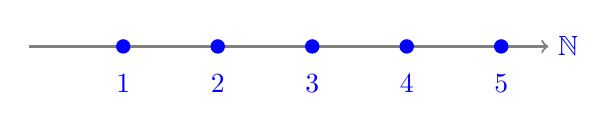
\begin{tikzpicture}[scale=1.2]
    \draw[->, thick, gray] (0,0) -- (5.5,0);
    \foreach \x in {1,2,3,4,5} {
        \filldraw[blue] (\x,0) circle (2pt);
        \node[below, blue] at (\x,-0.2) {$\x$};
    }
    \node[right, blue] at (5.5, 0) {$\mathbb{N}$};
\end{tikzpicture}
\end{center}

Šioje aibėje galime laisvai sudėti ir dauginti. Tačiau pabandykime išspręsti lygtį:
\[ x + 3 = 2. \]
Koks natūralusis skaičius, pridėtas prie trijų, duos du? Tokio skaičiaus aibėje $\mathbb{N}$ nėra. Mums prireikė naujų skaičių.

\subsection{Sveikieji skaičiai ($\mathbb{Z}$)}

Kad išspręstume lygtį $x + 3 = 2$, mums prireikė neigiamų skaičių ir nulio.

\begin{definition}
\vocab{Sveikieji skaičiai} -- tai visi natūralieji skaičiai, jiems priešingi (neigiami) skaičiai ir nulis. Žymima raide $\mathbb{Z}$ (iš vokiečių kalbos žodžio \textit{Zahlen} -- skaičiai).
\[ \mathbb{Z} = \{\dots, -3, -2, -1, 0, 1, 2, 3, \dots\} \]
\end{definition}

Skaičių ašyje prie jau turimų natūraliųjų skaičių (mėlynų) pridedame naujus, sveikuosius skaičius (raudonus), kurie tęsiasi į kairę. 
Pastebėkite, kad visi natūralieji skaičiai yra ir sveikieji skaičiai, todėl galime užrašyti: $\mathbb{N} \subset \mathbb{Z}$.

\begin{center}
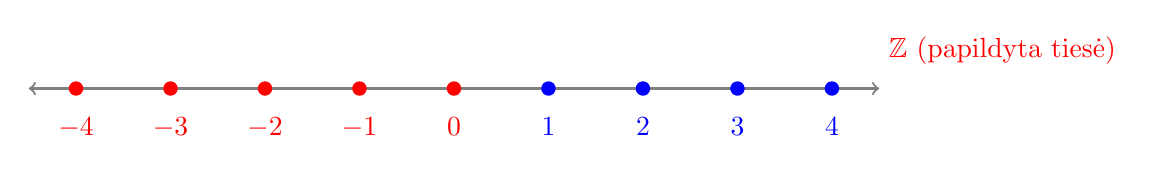
\begin{tikzpicture}[scale=1.2]
    \draw[<->, thick, gray] (-4.5,0) -- (4.5,0);
    % Natūralieji (senieji)
    \foreach \x in {1,2,3,4} {
        \filldraw[blue] (\x,0) circle (2pt);
        \node[below, blue] at (\x,-0.2) {$\x$};
    }
    % Naujieji (nulis ir neigiami)
    \foreach \x in {-4,-3,-2,-1,0} {
        \filldraw[red] (\x,0) circle (2pt);
        \node[below, red] at (\x,-0.2) {$\x$};
    }
    \node[right, red] at (4.5, 0.4) {$\mathbb{Z}$ (papildyta tiesė)};
\end{tikzpicture}
\end{center}

Lygtis $x + 3 = 2$ dabar turi sprendinį: $x = -1$. Bet pabandykime išspręsti kitą lygtį:
\[ 2 \cdot x = 3. \]
Koks sveikasis skaičius, padaugintas iš dviejų, duoda tris? Tokio skaičiaus vėl nėra. Tarpuose tarp sveikųjų skaičių vis dar tuščia!

\subsection{Racionalieji skaičiai ($\mathbb{Q}$)}

Dalybos problemai išspręsti prireikė trupmenų. 

\begin{definition}
\vocab{Racionalieji skaičiai} -- tai skaičiai, kuriuos galima užrašyti paprastąja trupmena $\frac{m}{n}$, kur $m \in \mathbb{Z}$ ir $n \in \mathbb{N}$. Žymima raide $\mathbb{Q}$ (iš italų kalbos žodžio \textit{quoziente} arba anglų \textit{quotient} -- dalmuo).
\end{definition}

Mūsų skaičių tiesėje atsiranda be galo daug naujų taškų (žalių) tarp sveikųjų skaičių. Kiekvieną natūralųjį ir sveikąjį skaičių galima užrašyti trupmena, kurios vardiklis yra $1$. Pavyzdžiui,
\[ 3 = \frac{3}{1}, \qquad 0 = \frac{0}{1}, \qquad -5 = \frac{-5}{1}. \]
Todėl visi natūralieji ir sveikieji skaičiai yra racionalieji skaičiai, o poaibių ryšį galime užrašyti taip:
\[ \mathbb{N} \subset \mathbb{Z} \subset \mathbb{Q}. \]

\begin{center}
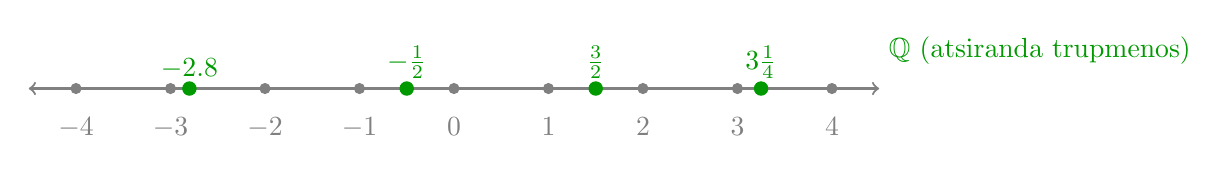
\begin{tikzpicture}[scale=1.2]
    \draw[<->, thick, gray] (-4.5,0) -- (4.5,0);
    % Sveikieji
    \foreach \x in {-4,-3,-2,-1,0,1,2,3,4} {
        \filldraw[gray] (\x,0) circle (1.5pt);
        \node[below, gray] at (\x,-0.2) {$\x$};
    }
    % Racionalieji (nauji)
    \filldraw[green!60!black] (1.5,0) circle (2pt) node[above] {$\frac{3}{2}$};
    \filldraw[green!60!black] (-0.5,0) circle (2pt) node[above] {$-\frac{1}{2}$};
    \filldraw[green!60!black] (3.25,0) circle (2pt) node[above] {$3\frac{1}{4}$};
    \filldraw[green!60!black] (-2.8,0) circle (2pt) node[above] {$-2.8$};
    
    \node[right, green!60!black] at (4.5, 0.4) {$\mathbb{Q}$ (atsiranda trupmenos)};
\end{tikzpicture}
\end{center}

Dabar lygtis $2 \cdot x = 3$ turi sprendinį $x = \frac{3}{2}$. Tiesė atrodo tanki, bet ar ji visiškai pilna?

\subsection{Iracionalieji skaičiai ($\mathbb{I}$)}

Geometrai greitai susidūrė su problema: kvadrato, kurio kraštinė lygi $1$, įstrižainės ilgis $x$ tenkina lygtį:
\[ x^2 = 2. \]
Ar egzistuoja tokia trupmena, kurią pakėlus kvadratu gautume tiksliai $2$? 

Norėdami išsiaiškinti, ar $\sqrt{2}$ yra racionalusis skaičius, galime pasirinkti vieną iš dviejų kelių. Pirmasis kelias būtų pabandyti $\sqrt{2}$ išreikšti trupmena ir tiesiogiai rasti tokius skaitiklį bei vardiklį. Tačiau iš anksto nežinome, kokia tai galėtų būti trupmena.

Todėl pasirinksime kitą kelią -- \textbf{prieštaros metodą}. Iš pradžių padarysime prielaidą, kad mūsų teiginys yra priešingas tam, ką norime įrodyti: tarkime, kad $\sqrt{2}$ yra racionalusis skaičius. Jeigu ši prielaida teisinga, iš jos turime gauti logiškai teisingas išvadas. Tačiau jeigu prielaida klaidinga, anksčiau ar vėliau turėtume gauti prieštarą, tai yra neįmanomą arba nelogišką išvadą. Tuomet suprasime, kad pradinė prielaida buvo klaidinga.

Taigi prieštaros metodo schema yra tokia: \textbf{tarkime priešingai, nuosekliai samprotaukime ir, gavę prieštarą, atmeskime pradinę prielaidą}.

\begin{proposition}
$\sqrt{2}$ nėra racionalusis skaičius.
\end{proposition}

\begin{proof}
Pasirinkome prieštaros metodą. Tarkime priešingai: $\sqrt{2}$ yra racionalusis skaičius. Tuomet jį galima užrašyti trupmena
\[
\sqrt{2}=\frac{m}{n},
\]
kur $m$ ir $n$ yra sveikieji skaičiai, $n\neq 0$, o trupmena yra sutrumpinta iki galo, t. y. $m$ ir $n$ neturi bendrų daliklių, didesnių už $1$.

Pakėlę abi lygybės puses kvadratu, gauname:
\[
2=\frac{m^2}{n^2},
\qquad 2n^2=m^2.
\]
Vadinasi, $m^2$ yra lyginis skaičius. Jei skaičiaus kvadratas yra lyginis, tai ir pats skaičius yra lyginis, todėl $m=2k$ su tam tikru sveikuoju skaičiumi $k$.

Įstatę $m=2k$ į lygybę $2n^2=m^2$, gauname:
\[
2n^2=(2k)^2=4k^2,
\qquad n^2=2k^2.
\]
Taigi $n^2$ yra lyginis, todėl ir $n$ yra lyginis.

Gavome, kad ir $m$, ir $n$ yra lyginiai. Tačiau pradžioje tarėme, kad skaičiai $m$ ir $n$ neturi bendro daliklio, išskyrus $1$. Dabar matome, kad jų bendras daliklis yra $2$. Tai yra prieštara.

Vadinasi, prielaida, kad $\sqrt{2}$ yra racionalusis skaičius, buvo klaidinga. Todėl $\sqrt{2}$ nėra racionalusis skaičius.
\end{proof}

Pasirodė, kad skaičių tiesėje tarp trupmenų vis dar yra begalybė „tuščių tarpų“! Šiuos tarpus užpildo iracionalieji skaičiai.

\begin{definition}
\vocab{Iracionalieji skaičiai} -- tai skaičiai, kurių negalima užrašyti paprastąja trupmena. Ši aibė dažnai žymima raide $\mathbb{I}$ (iš lotynų \textit{irrationalis} --  neapskaičiuojamas). Jų dešimtainė išraiška yra begalinė ir neperiodinė.
\end{definition}

\subsection{Realieji skaičiai ($\mathbb{R}$)}

Prireikė sujungti racionaliuosius ($\mathbb{Q}$) ir iracionaliuosius ($\mathbb{I}$) skaičius į vieną didelę šeimą.

\begin{definition}
\vocab{Realieji skaičiai} -- tai visi racionalieji ir iracionalieji skaičiai kartu paėmus. Žymima raide $\mathbb{R}$ (iš lotynų kalbos žodžio \textit{realis} -- tikras, realus). 
\end{definition}

Kai prie trupmenų pridedame iracionaliuosius skaičius (pvz., $\sqrt{2}$, $\pi$), realieji skaičiai \textbf{visiškai užpildo skaičių tiesę}. Nelieka nė vieno tuščio taško -- tiesė tampa ištisine, nenutrūkstančia linija (pažymėta violetine spalva).

Kadangi visi natūralieji ir sveikieji skaičiai yra racionalieji, o visi racionalieji skaičiai yra realieji, gauname grandinę:
\[ \mathbb{N} \subset \mathbb{Z} \subset \mathbb{Q} \subset \mathbb{R}. \]

\begin{center}
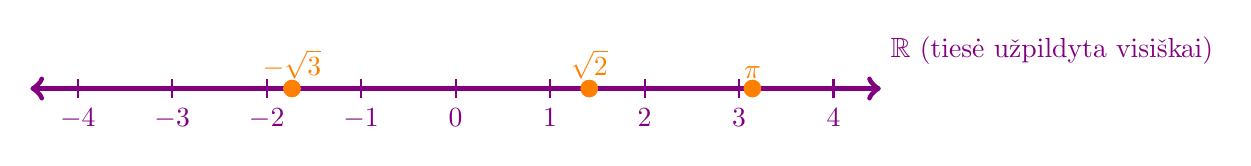
\begin{tikzpicture}[scale=1.2]
    % Ištisinė tiesė reiškia realiuosius
    \draw[<->, line width=2pt, violet] (-4.5,0) -- (4.5,0);
    \foreach \x in {-4,-3,-2,-1,0,1,2,3,4} {
        \draw[thick, violet] (\x,0.1) -- (\x,-0.1) node[below] {$\x$};
    }
    % Iracionalieji
    \filldraw[orange] (1.414,0) circle (2.5pt) node[above] {$\sqrt{2}$};
    \filldraw[orange] (3.141,0) circle (2.5pt) node[above] {$\pi$};
    \filldraw[orange] (-1.732,0) circle (2.5pt) node[above] {$-\sqrt{3}$};
    
    \node[right, violet] at (4.5, 0.4) {$\mathbb{R}$ (tiesė užpildyta visiškai)};
\end{tikzpicture}
\end{center}


\section{Kompleksiniai skaičiai: nuo tiesės prie plokštumos}

Atrodo, kad su realiaisiais skaičiais matematikos problemos išspręstos. Bet pabandykime išspręsti šią lygtį:
\[ x^2 = -1. \]
Mes žinome, kad bet kokį realųjį skaičių pakėlus kvadratu, rezultatas visada yra teigiamas arba nulis (pvz., $(-1)^2 = 1$). Realiųjų skaičių tiesėje tiesiog nėra tokio skaičiaus, kurio kvadratas būtų lygus $-1$. 

Kadangi skaičių tiesė jau yra \textbf{visiškai užpildyta}, mes negalime joje rasti vietos jokiam naujam skaičiui. Ką daryti? 

Nubrėžkime naują, \textbf{vertikalią ašį}, kuri kerta mūsų senąją realiųjų skaičių tiesę ties nuliu. Šią naują ašį pavadinsime \textbf{menamąja ašimi} ir žymėsime trumpiniu \textbf{Im} (nuo angliško žodžio \textit{imaginary} -- įsivaizduojamas, menamas).

\begin{center}
\begin{tikzpicture}[scale=1.25]
    % Realiųjų ir menamųjų skaičių ašys
    \draw[<->, thick, violet] (-3.5,0) -- (3.5,0)
        node[right, text=black] {Re ($\mathbb{R}$ ašis)};
    \draw[<->, thick, cyan!80!black] (0,-2.2) -- (0,2.2)
        node[above, text=black] {Im (menamoji ašis)};

    \foreach \x in {-3,-2,-1,1,2,3}
        \draw[thick, violet] (\x,0.1) -- (\x,-0.1) node[below] {$\x$};
    \node[below left] at (0,0) {$0$};
\end{tikzpicture}
\end{center}

Tegul tas ieškomas skaičius, kurio kvadratas yra $-1$, vadinasi $i$ (pirmoji žodžio \textit{imaginary} raidė). Šį skaičių pažymėsime vertikalioje ašyje lygiai toje pačioje vietoje, kur horizontalioje ašyje žymėdavome paprastą vienetą -- kaip $1i$ (arba tiesiog $i$).

\begin{center}
\begin{tikzpicture}[scale=1.25]
    % Realiųjų ir menamųjų skaičių ašys
    \draw[<->, thick, violet] (-3.5,0) -- (3.5,0)
        node[right, text=black] {Re ($\mathbb{R}$ ašis)};
    \draw[<->, thick, cyan!80!black] (0,-2.2) -- (0,2.2)
        node[above, text=black] {Im (menamoji ašis)};

    \foreach \x in {-3,-2,-1,1,2,3}
        \draw[thick, violet] (\x,0.1) -- (\x,-0.1) node[below] {$\x$};
    \foreach \y in {-2,-1,1,2}
        \draw[thick, cyan!80!black] (0.1,\y) -- (-0.1,\y) node[left] {$\y i$};
    \node[below left] at (0,0) {$0$};
    \filldraw[red] (0,1) circle (2pt);
\end{tikzpicture}
\end{center}

\begin{definition}
\vocab{Menamasis vienetas} -- tai specialus įsivaizduojamas skaičius, žymimas raide $i$, kurio kvadratas lygus $-1$.
\[ i^2 = -1. \]
\end{definition}

Iššokę iš tiesės į plokštumą mes gauname naują, pačią didžiausią skaičių aibę. 

\begin{definition}
\vocab{Kompleksiniai skaičiai} -- tai skaičiai, kuriuos galima užrašyti forma $z = a + bi$, kur $a$ ir $b$ yra realieji skaičiai, o $i$ -- menamasis vienetas. Čia $a$ vadinama realiąja dalimi, o $b$ -- menamąja dalimi. Ši aibė žymima raide $\mathbb{C}$ (iš lotynų \textit{complexus} -- sudėtinis, sujungtas iš dviejų dalių).
\end{definition}

Visi realieji skaičiai yra kompleksinių skaičių atvejis, kai menamoji dalis lygi nuliui. Kitaip tariant, kompleksinis skaičius $z=a+bi$ yra realusis skaičius tada, kai $b=0$, todėl $z=a$.

Taigi visų nagrinėtų skaičių aibių ryšį galime užrašyti viena grandine:
\[ \mathbb{N} \subset \mathbb{Z} \subset \mathbb{Q} \subset \mathbb{R} \subset \mathbb{C}. \]

\section{Kompleksinių skaičių vaizdavimas}

Kompleksinį skaičių $z = a + bi$ galime įsivaizduoti kaip tašką koordinačių plokštumoje, kurio koordinatės yra $(a; b)$. 
Skaičius $a$ žymimas ant horizontalios (realiosios) ašies, o skaičius $b$ -- ant vertikalios (menamosios) ašies, prirašant raidę $i$.

\begin{example}
Pažymėkite kompleksinius skaičius kompleksinėje plokštumoje:
\begin{tasks}[label=(\alph*), label-offset=0.9em](1)
    \task $z_1 = 3 + 2i$
    \task $z_2 = -4 + i$
    \task $z_3 = 1 - 3i$
    \task $z_4 = 4i$
\end{tasks}
\end{example}
\begin{solution}
Pirmiausia nubrėžiame kompleksinę plokštumą, t. y. realiąją ir menamąją ašis. Tada pradedame žymėti kompleksinius skaičius.

\begin{tasks}[label=(\alph*), label-offset=0.9em](1)
    \task Skaičiaus $z_1 = 3 + 2i$ realioji dalis yra $3$, o menamoji dalis yra $2$, todėl jo koordinatės yra $(3; 2)$.
    \task Skaičiaus $z_2 = -4 + i$ realioji dalis yra $-4$, o menamoji dalis yra $1$, todėl jo koordinatės yra $(-4; 1)$.
    \task Skaičiaus $z_3 = 1 - 3i$ realioji dalis yra $1$, o menamoji dalis yra $-3$, todėl jo koordinatės yra $(1; -3)$.
    \task Skaičiaus $z_4 = 4i = 0 + 4i$ realioji dalis yra $0$, o menamoji dalis yra $4$, todėl jo koordinatės yra $(0; 4)$.
\end{tasks}

\begin{center}
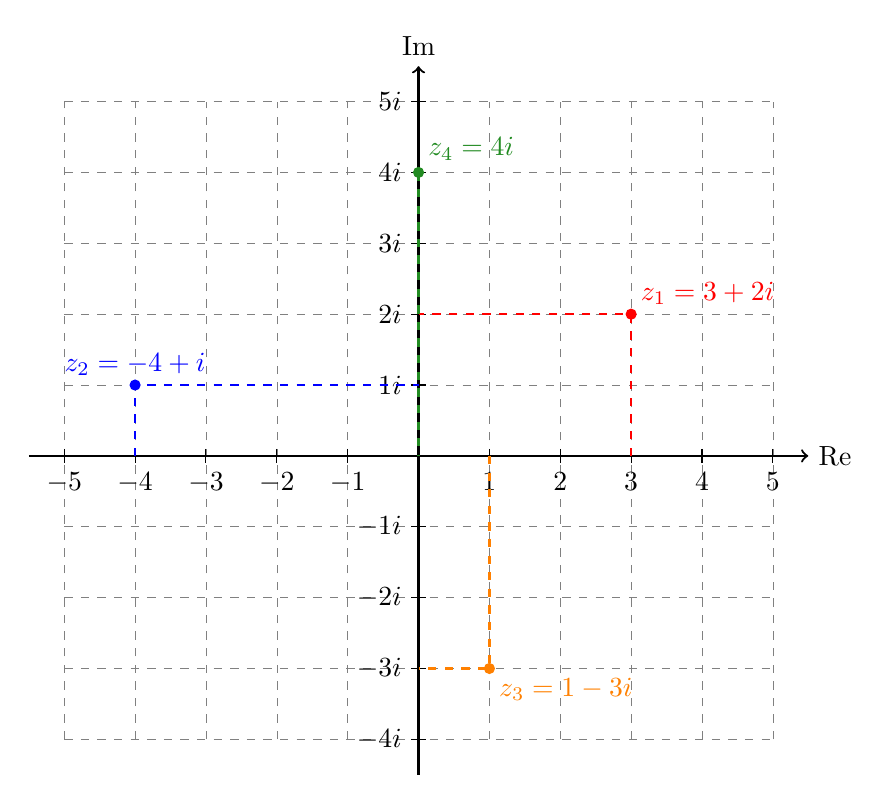
\begin{tikzpicture}[scale=0.9]
    \draw[step=1cm,gray,very thin, dashed] (-5,-4) grid (5,5);
    \draw[->, thick] (-5.5,0) -- (5.5,0) node[right] {Re};
    \draw[->, thick] (0,-4.5) -- (0,5.5) node[above] {Im};
    
    \foreach \x in {-5,...,-1,1,2,...,5}
        \draw (\x,0.1) -- (\x,-0.1) node[below] {$\x$};
    \foreach \y in {-4,-3,-2,-1,1,2,3,4,5}
        \draw (0.1,\y) -- (-0.1,\y) node[left] {$\y i$};
    
    % Taškas z_1
    \filldraw[red] (3,2) circle (2pt) node[anchor=south west] {$z_1 = 3 + 2i$};
    \draw[thick, red, dashed] (3,0) -- (3,2) -- (0,2);
    
    % Taškas z_2
    \filldraw[blue] (-4,1) circle (2pt) node[anchor=south] {$z_2 = -4 + i$};
    \draw[thick, blue, dashed] (-4,0) -- (-4,1) -- (0,1);

    % Taškas z_3
    \filldraw[orange] (1,-3) circle (2pt) node[anchor=north west] {$z_3 = 1 - 3i$};
    \draw[thick, orange, dashed] (1,0) -- (1,-3) -- (0,-3);

    % Taškas z_4
    \filldraw[ForestGreen] (0,4) circle (2pt) node[anchor=west,yshift=3mm] {$z_4 = 4i$};
    \draw[thick, ForestGreen, dashed] (0,4) -- (0,0);
\end{tikzpicture}
\end{center}
\end{solution}
\newpage
\section{Uždaviniai}

\begin{problem}
Nustatykite, kokioms skaičių aibėms ($\mathbb{N}$, $\mathbb{Z}$, $\mathbb{Q}$, $\mathbb{I}$, $\mathbb{R}$ ar $\mathbb{C}$) priklauso kiekvienas nurodytas skaičius. Išvardykite visas tinkamas aibes.
\begin{tasks}[label={(\arabic*)}, label-offset=0.9em](5)
    \task $1$
    \task $12$
    \task $0$
    \task $-7$
    \task $\frac{1}{2}$
    \task $-\frac{7}{3}$
    \task $1{,}25$
    \task $\sqrt{2}$
    \task $\pi$
    \task $-\sqrt{5}$
    \task $2+i$
    \task $-3+4i$
    \task $-i$
    \task $5i$
    \task $0{,}125$
    \task $\frac{11}{2}$
    \task $-12$
    \task $\sqrt{7}$
    \task $1-2i$
    \task $-6+i$
\end{tasks}
\end{problem}

\setcounter{problem}{2}
\begin{problem}
Užrašykite kompleksinį skaičių $z = a + bi$, jei žinomos jo realioji ($a$) ir menamoji ($b$) dalys:
\begin{tasks}[label={(\arabic*)}, label-offset=0.9em](2)
    \task $a = 3$, $b = 4$
    \task $a = -2$, $b = 1$
    \task $a = 0$, $b = -5$
    \task $a = 7$, $b = 0$
\end{tasks}
\end{problem}

\setcounter{problem}{3}
\begin{problem}
Išrašykite šių kompleksinių skaičių koordinates koordinačių plokštumoje $(x; y)$ pavidalu. (Savarankiškai pasižymėkite jas sąsiuvinio brėžinyje).
\begin{tasks}[label={(\arabic*)}, label-offset=0.9em](2)
    \task $z = 4 + 3i$
    \task $z = -3 + 2i$
    \task $z = -1 - 4i$
    \task $z = 5i$
    \task $z = -2$
    \task $z = 2 - i$
    \task $z = 1 + i$
    \task $z = -4 - 2i$
    \task $z = 5i$
    \task $z = -3i$
\end{tasks}
\end{problem}

\newpage
\answerssection

\begin{problem} \phantom{text}
\begin{tasks}[label={(\arabic*)}, label-offset=0.9em](5)
    \task $\mathbb{N},\mathbb{Z},\mathbb{Q},\mathbb{R},\mathbb{C}$
    \task $\mathbb{N},\mathbb{Z},\mathbb{Q},\mathbb{R},\mathbb{C}$
    \task $\mathbb{Z},\mathbb{Q},\mathbb{R},\mathbb{C}$
    \task $\mathbb{Z},\mathbb{Q},\mathbb{R},\mathbb{C}$
    \task $\mathbb{Q},\mathbb{R},\mathbb{C}$
    \task $\mathbb{Q},\mathbb{R},\mathbb{C}$
    \task $\mathbb{Q},\mathbb{R},\mathbb{C}$
    \task $\mathbb{I},\mathbb{R},\mathbb{C}$
    \task $\mathbb{I},\mathbb{R},\mathbb{C}$
    \task $\mathbb{I},\mathbb{R},\mathbb{C}$
    \task $\mathbb{C}$
    \task $\mathbb{C}$
    \task $\mathbb{C}$
    \task $\mathbb{C}$
    \task $\mathbb{Q},\mathbb{R},\mathbb{C}$
    \task $\mathbb{Q},\mathbb{R},\mathbb{C}$
    \task $\mathbb{Z},\mathbb{Q},\mathbb{R},\mathbb{C}$
    \task $\mathbb{I},\mathbb{R},\mathbb{C}$
    \task $\mathbb{C}$
    \task $\mathbb{C}$
\end{tasks}
\end{problem}

\setcounter{problem}{2}
\begin{problem} \phantom{text}
\begin{tasks}[label={(\arabic*)}, label-offset=0.9em](2)
    \task $z = 3 + 4i$;
    \task $z = -2 + i$;
    \task $z = -5i$;
    \task $z = 7$.
\end{tasks}
\end{problem}

\setcounter{problem}{3}
\begin{problem} \phantom{text}
\begin{tasks}[label={(\arabic*)}, label-offset=0.9em](2)
    \task $(4; 3)$;
    \task $(-3; 2)$;
    \task $(-1; -4)$;
    \task $(0; 5)$;
    \task $(-2; 0)$;
    \task $(2; -1)$;
    \task $(1; 1)$;
    \task $(-4; -2)$;
    \task $(0; 5)$;
    \task $(0; -3)$.
\end{tasks}
\end{problem}

\end{document}